\documentclass[12pt]{article}

% links
\usepackage{hyperref}
% foreach macro
\usepackage{pgffor}
\usepackage{array}
\usepackage{subcaption}
\usepackage{graphicx}
\usepackage{amsmath}
\usepackage{bookmark}
\usepackage{caption}
\usepackage{float}
\usepackage[french]{babel}
\usepackage[T1]{fontenc}
\usepackage{bm}
\usepackage{newtxtext,newtxmath}
\usepackage[
    left = \flqq{},% 
    right = \frqq{},% 
    leftsub = \flq{},% 
    rightsub = \frq{} %
]{dirtytalk}
\DeclareUnicodeCharacter{2212}{-}
\begin{document}

\title{Tesi}

\author{Iris Dania Jimenez}

\maketitle

\tableofcontents
\newpage

\section{Introduzione}

In questa tesi si è sviluppato il concetto di \say{competitività} tra diversi stati a partire dal Regional Innovation Scoreboard(RIS),
con lo scopo di creare una classifica dei paesi europei più competitivi, per poterli poi comparare tra di loro.  
Il RIS è dataset, pubblicato ogni anno a partire dal 2014 dall'Unione Europea, composto da un insieme di indicatori che valutano 
le performance sotto diversi punti di vista dei vari stati Europei.  \\
\\
Il World Economic Forum definisce la competitività tra paesi come \linebreak
$\textit{"l'insieme di istituzioni e politiche che determinano 
il livello di produttività $\newline$ di un paese"}$, mentre The Oxford Dictionary la definisce come \linebreak
$\textit{"l'abilità di un'economia di aumentare la domanda e mantenere alte le esportazioni"}$. \\
Entrambe queste definizioni non sono molto precise, in quanto non individuano quali siano i fattori determinanti che contribuiscono a 
formare la competitività di un paese, ma invece indicano delle metriche per cercare di misurarla, come la produttivà e il livello 
di esportazioni di un paese. \\
Inoltre, entrambe queste definizioni si concentrano fortemente sull'aspetto economico della competitività di un paese, tralasciando altri fattori. 
Intuitivamente quando pensiamo ad un paese \say{competitivo}, la sfera economica risulta essere certamente importante e determinante nel 
definire il livello di competitività di uno stato, ma non è l'unico aspetto da considerare. Vi sono, infatti, altri fattori che
influiscono sul concetto di \say{competitività}, i quali però non risultano essere altrettanto discussi e analizzati dalle 
istituzioni.  \\
Con questa tesi il mio obiettivo invece è quello di sviluppare il concetto di \say{competitività} con lo scopo di indivuare quali sono i 
fattori che la determinano e che la influenzano, utilizzando gli indicatori presenti nel Regional Innovation Scoreboard, per infine 
creare una classifica dei diversi stati europei che mostri quali sono i paesi più \say{competitivi}. \\
Una classifica multidimensionale sulla competitività può aiutare le istituzioni a comprendere quali sono gli elementi che la determinano e 
che la influenzano, andando così a fornire un supporto nel capire quali sono i settori ed i paesi che maggiormente necessitano di 
aiuti e finanziamenti per aumentare la loro competitività a livello europeo. \\
Queste informazioni possono fornire validi ed efficaci insights con il fine di avvantaggiare e favorire i paesi europei a livello 
internazionale, sotto un'ottica di cooperazione e solidarietà tra stati membri. \\
\\
Prendendo in considerazione più dimensioni, oltre a quella prettamente economica, risulta assai più complesso e meno intuitivo creare
una classifica della \say{competitività} tra paesi, questo perchè alcuni stati potrebbero avere performance maggiori su alcune dimensioni e minori 
su altre, andando così a creare contrasti difficilmente risolvibili. Date queste complessità ho utlizzato la teoria degli ordinamenti parzialmente ordinati(poset), che ha proprio lo scopo di formalizzare e 
generalizzare il concetto di \say{ordinamento}. I poset sono $\textit{parzialemente ordinati}$ perchè non ogni coppia di elementi è 
comparabile, ossia vi sono delle incomparabilità, come nel caso in cui un paese abbia dei valori maggiori su alcuni indicatori e minori 
su altri. Ma nonostante queste difficoltà gli ordinamenti parzialemente ordinati sono in grado di fornire un ordinamento
$\textit{totalmente ordinato}$, in cui ogni coppia di elementi, stati nel nostro caso, è comparabile. \\
Nella seconda sezione di questa tesi descriverò la teoria degli ordinamenti parzialmente ordinati e spiegherò come nonostante 
sussistano delle incomparabilità tra gli elementi di un dataset, i poset sono in grado di fornire comununque un unico ordinamento finale. Successivamente 
presenterò i dati utilizzati e descriverò le principali tecniche statiche e computazionali utilizzate nell'analisi dei dati. Infine 
presenterò i risultati e le conclusioni delle analisi. 




\newpage


\section{Insiemi parzialemente ordinati}

I poset(partially ordered set) sono insiemi parzialmente ordinati utilizzati in matematica, in 
particolare nella teoria degli ordini, 
per effettuare una riduzione della dimensionalità su dati di tipo ordinale. Lo scopo dei poset quindi,
risulta essere quello di ridurre ad un ranking, quindi una struttura di tipo unidimensionale, un insieme di indicatori ordinali 
i quali si presentano come degli oggetti multidimensionali. \\
Gli indicatori di tipo ordinale sono ampiamente diffusi sopratutto in campo sociale e vengono 
utilizzati per esprimere idee e nozioni che per loro natura non posso essere rigorosamente ordinati secondo 
una scala metrica. Per esempio, i concetti legati alla sfera emotiva come la felicità, la soddisfazione ed il benessere vengono espressi tramite indicatori di questo tipo. Fanno parte dei dati ordinali 
tutti quegli indicatori che richiedono di esprimere un giudizio o un'opinione.\\
Il problema che si incontra con questo tipo di dati è quello di effetturare un'analisi statistica
multivariata su un tipo di dato \say{non-matematico}. Per ovviare a questo problema molto spesso si 
cerca di trasformare in una qualche maniera il dato ordinale in un dato numerico, per poi procedere 
con le usuali tecniche di analisi statistica che meglio si conciliano con i fini della ricerca. \\
Tralasciando il discorso su che tipo di risultati le canoniche tecniche di analisi possono 
produrre su dati la cui vera natura è non numerica, il problema che si pone è un altro e di natura 
ben più profonda; perchè dover necessariamente trasformare il dato? Questa idea si basa sul concetto 
che la forma in cui il dato viene naturalmente espresso sia in qualche modo sub-ottimale e di minor 
qualità rispetto al classico dato numerico. Eppure nella nostra quotidiana esperienza tutti noi facciamo
largamente uso di questo tipo di dato. Nella vita di tutti i giorni non esprimiamo i concetti e le nostre esperienze
in numeri ma tramite le nozioni di \say{migliore} o \say{peggiore}, \say{buono} e \say{meno buono}, \say{bello} e \say{brutto}. 
Perrchè allora cercare di forzare e trasformare la vera natura del dato? Perchè assumere che la vera 
variabile latente sottostance al concetto che vogliamo esprimere sia numerica? Soprattutto, alla luce di 
questi nuovi concetti sarebbe ancora ragionevolmente sensato e attendibile 
interpretare come veritiero ciò che otteniamo come risultato? \\
Un nuovo e differente approccio è quello di cercare di mappare i dati come sono senza trasformazioni, 
ed è in questo campo che vengono utilizzati i poset. Tramite la teoria degli ordinamenti parzialmente
ordinati si cerca di costruire una grammatica del dato multidimensionale che preservi la natura 
ordinale del dato. 

\subsection{Definizione}

Sia X un insieme e sia $\leq$ una relazione binaria, tale che abbia le proprietà di;\\
\\
1) riflessività: x $\leq$ x, $\forall$ x $\in$ X\\
\\
2) antisimmetria: x $\leq$ y e y $\leq$ x $\Leftrightarrow$ x = y, $\forall$ x, y $\in$ X \\
\\
3) transitività: x $\leq$ y e y $\leq$ z $\Rightarrow$ x $\leq$ z, $\forall$ x, y, z $\in$ X\\
\\
Allora la coppia (X, $\leq$) è chiamata insieme parzialmente ordinato. \\
Pertanto un poset si presenta come une relazione binaria tra un insieme X e la relazione d'ordine 
$\leq$  con le proprietà sopraelencate di riflessività, antisimmetria e transitività.\\
La proprietà di riflessività ci garantisce che ogni elemento è relazionato con se stesso, 
mentre la proprietà di antisimmetria assicura che qualunque siano gli elementi di x e y 
appartenenti all'insieme X, le relazioni  x $\leq$ y e y $\leq$ x non possono sussistere 
contemporaneamente quando x è diverso da y. Infine la proprietà di transitività afferma che 
se sussite una relazione tra x e y e, a sua volta, sussiste una relazione tra y e z, allora 
esisterà anche una relazione tra x e z, con x, y e z appartenenti allo stesso insieme X. 



\subsection{Diagramma di Hasse}

I poset possono essere rappresentati graficamente tramite il diagramma di Hasse, il quale prende il nome 
dal sui ideatore Helmut Hasse$\footnote[1]{Helmut Hasse fu un matematico tedesco che lavorò nel campo della teoria
algebrica dei numeri, fondamentali sono i suoi contributi alla teoria dei campi.}$(1898-1979). Esso si presenta come un grafo formato
 da un insieme di nodi uniti da archi orientati. Di seguito è riportato un esempio di un diagramma di Hasse. \\
 Sia P = (\{a, b, c, d, e, f, g, h, i, l\}, $\leq$) un insieme parzialmente ordinato. Un possibile diagramma di Hasse 
 associato può essere, il seguente; \\
 \begin{figure}[H]
    \centering
    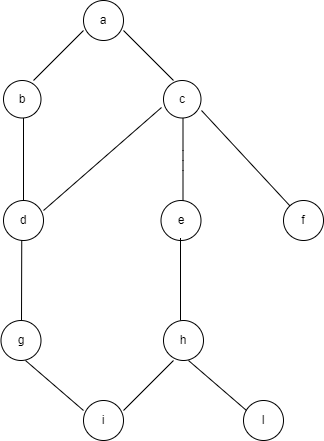
\includegraphics[scale=.5]{diagramma_hasse.png}
    \caption{Diagramma di Hasse del poset P}
\end{figure}

Il diagramma si legge dall'alto verso il basso e due generici elementi sono tra loro comparabili se 
risultano essere uniti da una sequenza discendente di archi, nel caso in cui questa sequenza discendente di 
archi non dovesse essere presente i due elementi sono incomparabili. \\
Nell'esempio proposto nella figura 1 \say{a} e \say{b} sono comparabili, mentre \say{b} e \say{f} sono incomparabili, 
in quanto non vi è una sequenza discendente di archi ad unire i due elementi. \\
In questo modo il poset può essere interpretato come un insieme di coppie di elementi che possono
essere tra loro comparabili o non comparabili. \\
Ai fini di comprendere appieno il diagramma di Hasse è necessario introdurre un ulteriore concentto
di fondamentale importanza per gli ordinamenti parzialemente ordinati; la nozione di copertura. \\
\\
L'idea sottostante alla relazione di copertura è che un elemento $\textit{domina}$ un'altro elemento se e solo se vi è
una successione di \say{coperture} che lega i due elementi. Nell'esempio in figura 1 \say{a} copre \say{b} perchè
\say{sta sopra} a quest'ultimo. A sua volta \say{b} domina \say{d} e per la proprietà di transitività a sua volta, \say{a}
domina \say{d}. Si formano così insieme di coppie comparabili o incomparabili, ed in tal senso possiamo dire che la relazione 
di copertura genera la relazione d'ordine, dato che quest'ultima è ottenuta seguendo transitivamente gli archi che collegano i punti. \\
Quando un elemento domina tutti gli altri assume il nome di $\textit{massimo}$. In figura 1 \say{a} è un massimo, appunto perchè
domina tutti gli altri elementi. Nel diagramma di Hasse soprarappresentato, non sono presenti $\textit{minimi}$, in quanto nessun elemento viene dominato
da tutti, ma sono invece presenti dei $\textit{minimali}$, elementi che non dominano nessuno ma non sono dominati da tutti. 
Nell'esempio illustrato i minimali risultano essere \say{f}, \say{i} ed \say{l}. \\
Una rappresentazione di un diagramma di Hasse in cui sono presenti $\textit{minimi}$ e $\textit{massimali}$, è la seguente;\\
\begin{figure}[H]
    \centering
    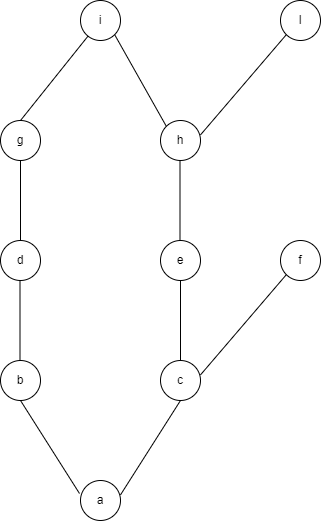
\includegraphics[scale=.5]{hasse2.png}
    \caption{Diagramma di Hasse del poset P}
\end{figure} 

In figura 2 \say{a} è un minimo, perchè viene dominato da tutti gli elementi, mentre \say{i}, \say{l}, \say{f} sono dei massimali,
in quanto non vengono dominati da nessuno ma non dominano tutti. \\
Un poset con un numero finito di elemento ammette sempre minimali e massimali, ma non sempre ha massimo o minimo. \\
\\ 
In un insieme parzialmente ordinato un sottoinsieme di elementi tutti fra loro comparabili viene chiamato $\textit{catena}$.
In figura 1 un esempio di catena è il sottoinsieme composto dai punti \say{a}-\say{b}-\say{d}-\say{g}-\say{i}\\
\begin{figure}[H]
    \centering
    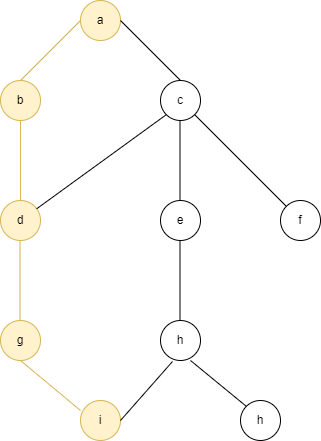
\includegraphics[scale=.5]{hasse_catena.png}
    \caption{Evidenziata una catena}
\end{figure}

Le anticatene invece sono sottoinsiemi costituiti da elementi tutti fra loro incomparabili. \\
\begin{figure}[H]
    \centering
    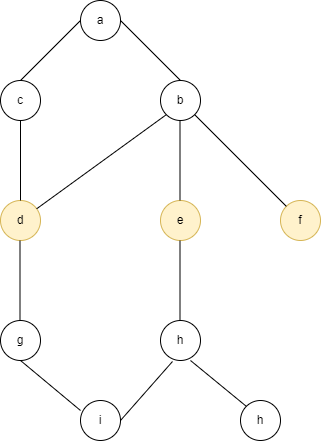
\includegraphics[scale=.5]{ant_catena.png}
    \caption{Evidenziata una anticatena}
\end{figure}

Le anticatene aggiungono ricchezza nella comprensione del dato ordinale poichè esprimono la nozione di $\textit{incomparabilità}$, propria 
dei dati non numerici. I dati di tipo ordinale presentano diverse e numerose sfaccetturare e sfumature che compongono il fenomeno in studio. 
Normalmente gran parte di questo tipo di informazione andrebbe persa con i classici approcci numerici, ma tramite gli insieme parzialmente 
ordinati siamo in grado di costruire un oggetto formale non euclideo in grado di catturare alcune caratteristiche importanti 
dei nostri dati e di ricavarne dell'informazione, senza trasformare e snaturare il dato dalla sua forma originaria con una conseguenza 
perdita di informazione.\\

\subsection{Estensioni lineari}

Un'estensione lineare è un ordinamento completo che contiene tutte le comparabilità del poset di input, cioè che è compatibile con esso. 
L'idea è quella di trasformare alcune incomparabilità in comparabilità, in modo tale da ottenere un ordinamento completo che contiene tutte 
le comparabilità del poset di input. Per ottenere questo risultato si aggiunge comparabilità al poset finchè non si ottiene un poset che non
può più essere esteso perchè è diventato lineare. \\
Gli oggetti che si creano da questo processo prendono il nome di $\textit{estensioni lineari}$. $\textit{Estensioni}$ poichè aggiungendo comparabilità
si estende l'insieme delle coppie comparabili del poset, $\textit{lineari}$ perchè non vi sono più incomparabilità. \\
Sia $P_1$ = (\{a, b, c, d, e\}, $\leq$) un poset, l'insieme delle sue estensioni lineari sono rappresentate in figura 5 insieme 
al poset stesso. 
\begin{figure}[H]
    \centering
    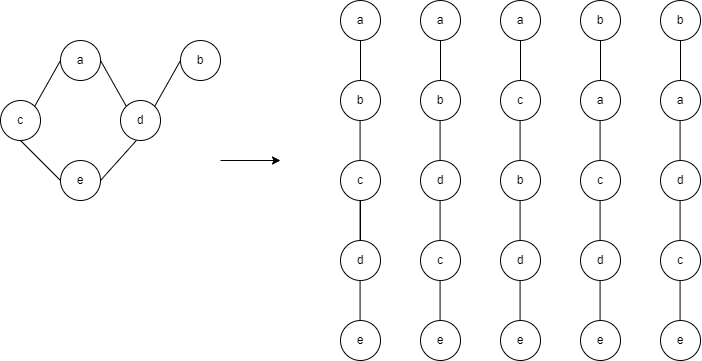
\includegraphics[scale=.5]{estensione_lin.png}
    \caption{Tutte le sole ed uniche estensioni lineari del poset $P_1$}
\end{figure}

Le estensioni lineari permettono di ricostruire univocamente il poset di partenza. Difatti, le comparabilità del poset sono tutte e solo le 
comparabilità comuni al suo insieme di estensioni lineari. Nell'esempio possiamo vedere come l'elemento \say{e}, il quale è un minimo, si trovi
sempre all'ultimo posto in tutte e cinque le differenti estensioni lineari, mentre gli elementi \say{a} e \say{b}, i quali sono entrambi due
massimali, siano sempre al primo posto nelle diverse estensioni lineari. L'elemento \say{a} domina più elementi di quanti non ne domini 
\say{b}, intuitivamente quindi anche se \say{a} e \say{b} non sono comparabili si sviluppa il concetto che \say{a} \say{è maggiore} in qualche modo
di \say{b}. Questa intuizione si riproduce nell'estensione lineare nel fatto che \say{a} è più spesso al primo posto rispetto all'elemento \say{b}. \\
Di fatto possiamo osservare come queste catene sono ottenute ordinando, in tutti i diversi possibili modi, le coppie incomparabili del poset
di partenza, senza però andare a modificare le comparabilità già esistenti.
Perciò possiamo affermare che un poset è equivalente alle sue estensioni estensioni
lineari, ed attraverso di esse siamo in grado di trasformare un problema descritto da una struttura complessa a più dimensioni in una
struttura unidimensionale più semplice. \\
In termini pratici ciò che si ottiene è che l'analisi statistica su un ordinamento parzialemente ordinato può, nella maggior parte dei casi,
essere ricondotta alle sue estensioni lineari, proprio grazie al fatto che queste individuano univocamente un poset. Come conseguenza, non si 
lavora più con degli oggetti multidimensionali, ma con degli ordinamenti completi semplici, i quali sono ricondicibili a variabili ordinali
multidimensionali. \\
\\
\\
Fin ora abbiamo introdotto il concetto di ordinamento parzialemente ordinato e le principali problematiche legate all'analisi di insiemi
di indicatori ordinali. I diagrammi di Hasse e le estensioni lineari sono differenti espressioni di un poset, che rappresentano e mantengono le 
fondamentali nozioni di comparabilità,  e di conseguenza di incomparabilità, che rendono i poset così particolari e non banali da analizzare e 
comprendere, sopratutto da un punto di vista matematico-statistico. Tuttavia questi elementi non bastano per avere una profonda comprensione
dell'argomento e
per effettuare una attenta analisi dei fenomeni qualitativi. Per questi motivi, sempre nell'ambito della toeria degli insiemi di cui fanno 
parte gli insiemi parzialemente ordinati vi sono altri elementi, che permettono, sempre mantenendo le nozioni di comparabilità ed incomparabilità,
di studiare e modelizzare il problema da una prospettiva matematica. \\
A differenza dei canonici metodi utilizzati per l'analisi di dati ordinali discussi precedentemente, le tecniche esposte di seguito hanno 
la peculiarità e la caratteristica di conservare l'ordine naturale dei dati ordinali. \\

\subsection{Rappresentazione matriciale di un insieme parzialmente ordinato}

Gli insiemi parzialmente ordinati possono essere rappresentati anche sotto forma matriciale, tramite le matrice Z di $\textit{dominanza}$
e la matrice G di $\textit{copertura}$. Di seguito vengono proposte le matrici G e Z per il poset $P_1$ rappresentato in figura 5. 
\begin{align}
    Z = 
    \left( \begin{array}{ccccc} 1 & 0 & 1 & 1 & 1 \\
        0 & 1 & 0 & 1 & 0\\
        1 & 0 & 1 & 0 & 1\\
        1 & 1 & 0 & 1 & 1\\
        1 & 0 & 1 & 1 & 1 \end{array} \right)
    \mbox{                  }
    G = 
    \left( \begin{array}{ccccc} 0 & 0 & 1 & 1 & 0 \\
        0 & 0 & 0 & 1 & 0\\
        1 & 0 & 0 & 0 & 1\\
        1 & 1 & 0 & 0 & 1\\
        0 & 0 & 1 & 1 & 0 \end{array} \right)
\end{align}
\\
Le colonne e le righe di ambe due le matrici rappresentano gli elementi del poset $P_1$ = (\{a, b, c, d, e\}, $\leq$) \\
La matrice di copertura G rappresenta lo scheletro della relazione d'ordine; presenta degli \say{1} se un elemento copre un 
altro e \say{0} altrimenti. Mentre la matrice di dominanza Z esprime la relazione d'ordine in senso vero e proprio, l'\say{1}
è presente se e solo se un elemento domina un altro e \say{0} altrimenti. Per definizione ogni elemento domina se stesso, 
perciò la matrice Z presenta tutti \say{1} sulla diagonale principale. \\
Nell'esempio soprariportato l'elemento $Z_{1,3}$ è uguale ad 1 perchè \say{a} domina \say{c}, e per transitività \say{a} domina
\say{e}, perciò l'elemento di $Z_{1,5}$, che rappresenta la coppia \say{a}-\say{e}, è sempre pari ad 1. 
Nella matrice G invece, dato che vengono riportati solo le relazioni di copertura l'elemento di $G_{1,3}$ è sempre pari ad 1, 
dato che \say{a} copre \say{c}, ma a differenza della relazione di dominanza, la relazione di copertura non è transitiva, 
perciò \say{a} non copre \say{e}, da cui l'elemento $G_{1,5}$ è pari a 0. \\
\\
Un'ulteriore rappresentazione matriciale dei poset si ha tramite la matrice di $\textit{mutual ranking probabilities}$
(MRP), la quale 
rappresenta al suo interno la quota di estensione lineare in cui un elemento domina un'altro. Infatti i valori all'interno della MRP si ottengono tenendo conto di quante volte l'elemento i-esimo 
domina l'elemento j-esimo. Pertanto
questa matrice esprime quanto intensamente i punti si dominano a vicenda, inoltre si nota anche che la matrice 
MRP identifica univocamente il poset in quanto \say{contiene} al proprio interno la matrice di dominanza 
Z. Di seguito vi è la rappresentazione della matrice M di mutual ranking probabilities
del poset $P_{1}$. 
\begin{align}
    M = 
    \left( \begin{array}{ccccc} 1 & 0,4 & 0 & 0 & 0 \\
        0,6 & 1 & 0,2 & 0 & 0\\
        1 & 0,8 & 1 & 0,4 & 0\\
        1 & 1 & 0,6 & 1 & 0\\
        1 & 1 & 1 & 1 & 1 \end{array} \right)
    \mbox{                  }
\end{align}
\\
Il valore di $M_{2,1}$ indica che nel 40\% delle volte l'elemento \say{b} domina \say{a}, allo stesso 
modo $M_{1,2}$ pari a 0,60 indica che nel 60\% delle volte \say{a} domina \say{b}. L'elemento \say{e}, è 
un minimo in quanto viene sempre dominato da tutti gli altri elementi, di conseguenza la quinta ed ultima riga della matrice 
presenta tutti valori unitari. Come nella matrice di dominanza Z anche nella matrice M ogni elemento
domina se stesso, perciò la diagonale principale presenta tutti gli elementi pari ad 1. 
In questo modo i valori all'interno della matriche di mutual ranking probabilities rappresentano proprio la quota 
di estensioni lineari che classificano l'elemento i-esimo sopra l'elemento j-esimo. 
La matrice di MRP risulta di fondamentale importanza perchè da essa si estrae successivamente l'informazione
necessaria per creare il ranking finale. L'idea alla base è che dato che ogni colonna esprime quanto 
quell'elemento domina gli altri, di conseguenza la media della colonna indicherà quanto un punto tende ad essere 
dominante rispetto a tutti gli altri punti e questo si presenta come un primo approccio alla costruzione di un ranking
finale. Il raking è una struttura unidimensionale perciò per ottenerlo si richiede di effetturare una 
riduzione della dimensionalità della matrice di MRP n $\times$k. Vi sono differenti tecniche che 
effettuano la riduzione della dimensionalità, ma la più utilizzata è la Singular Value Decomposition(SVD). 

\subsection{Singular Value Decomposition}


La $\textit{Singular Value Decomposition}$(SVD) è la soluzione ottimale a qualunque problema di approssimazione
dei dati di input. All'interno della teoria degli insiemi parzialmente ordinati è utilizzata per effettuare
un'ottimale riduzione della dimensionalità sulla matrice di mutual ranking probabilities. L'idea alla base 
è che una matrice X, complessa o reale di dimensione m$\times$n si possa scrivere come il prodotto
di tre matrici; U, D, V. 
\begin{align}
    X = UDV^t
\end{align}
dove; \\
\\
$\bullet$ U è una matrice n$\times$k le cui colonne sono ortonormali.\\
\\
$\bullet$ D è una matrice diagonale k$\times$k i cui elementi sulla diagonale sono i valori singolari della matrice X 
in ordine descrescente. \\
\\
$\bullet$ V è una matrice ortogonale k$\times$k le cui righe e colonne sono ortonormali. \\
\\
\\
Vi è una duplice interpretazione del risultato della decomposione a valori singolari. \\
In un primo caso possiamo effettuare la seguente assimilazione: 
\begin{align}
    X = UDV^t = AV^t
\end{align}
Con A = UD.\\
In questo caso ogni profilo della matrice X viene ricostruito come somma pesata delle righe 
ortonormali di $V^t$, con pesi nelle righe di A. Di conseguenza le righe di A appaiono come le coordinate 
delle righe della matrice X sulla base formata dalle righe ortornormali di $V^t$, ciò significa che 
esse contengono l'informazione necessaria a ricostruire le righe di X, una volta scelta la base di riferimento
data dalle righe di $V^t$. \\
Nel secondo caso possiamo vedere la decomposione a valori singolari nel seguente modo; 
\begin{align}
    X = UDV^t = UQ
\end{align}
Con Q = D$V^t$. \\
Così facendo la base vettoriale è data dalle righe di Q e le righe di U sono i coefficienti
della combinazione lineare che trovano le righe di X. Bisogna però porre attenazione al fatto che le 
righe di Q sono date dalle righe di $V^t$ moltiplicate per i valori singolari, perciò non sono più 
normalizzate. Questo non pone di per sè dei problemi, si tratta semplicemente di una scelta da compiere 
durante l'analisi. \\

Possiamo quindi affermare che tramite la decomposizione a valori singolari(3) noi identifichuamo le 
coordinate UD che costruiscono la matrice X sulla base formata dalle righe ortonormali di $V^t$, come 
risultato si ha che conoscere UD equivale a conoscere la matrice originale X. \\
\\
La SVD è definita come la $\textit{soluzione ottimale}$ a qualunque problema di approssimazione dei dati 
di input, ma cosa garantisce questa ottimalità della decomposizione a valori singolari rispetto ad altre 
tecniche di riduzione della dimensionalità? \\
La risposta si trova nel Teorema di Eckart-Young il quale stabilisce 
come costruire la matrice $\hat{X}$ che meglio approssima la matrice la matrice di input X nella 
norma di Frobenius$\footnote[1]{La norma di Frobenius $\Vert{M}_{F}$ $\Vert$ di una matrice M n$\times$k è definita come $\Vert{M}_{F}$ $\Vert$ = $\sqrt{Tr(M^tM)}$  }
$. Di seguito viene enunciato il teorema di Eckart-Young;\\
Sia X una matrice n$\times$k di rango k$\leq$ n, sia 0 < p $\leq$ k un intero fissato e sia X = UD$V^t$ la 
decomposzione a valori singolari di X. Indichiamo con $U_{[p]}$ la matrice n $\times$ p composta 
dalle prime p colonne di U, con $V_{[p]}$ la matrice k$\times$p composta dalle prime p colonne di V e con 
$D_{[p]}$ la matrice p$\times$p composta dalle prime p righe di e prime p colonne di D. La matrice 
\begin{align}
    \hat{X} = U_{[p]}D_{[p]}V_{[p]}^t = \sum_{i = 1}^{p} \sigma_{i} Z_{i}
\end{align}
minimizza la distanza $\Vert{X - \hat{X}}$$\Vert_{F}$ nell'insieme delle matrici n$\times$k, di rango p.\\ 
Con questa scrittura il Teorema di Eckart-Young ci permette di vedere la decomposizione a valori singolari come la sovrapposizione di p
layers(strati) tutti con rango unitario, pesati per i valori singolari $\sigma_{i}$. \\
\\
La SVD effettua la riduzione della dimensionalità ponendo a zero i valori oltre i p-esimo nella matrice D. Ciò significa che i valori da p+1
a k sono tutti nulli, di conseguenza restano solo k-p valori singolari non nulli. Ponendo a zero i valori singalori sulla matrice D vengono anche 
\say{annullati} i k-p valori delle colonne di U e righe di $V^t$. Di conseguenza la matrice $\hat{X}_{nxk}$ ha k colonne ma è di rango p. 
Come risultato ottengo che le righe della matrice approssimante $\hat{X}$ sono k dimensionali ma scrivibili come combinazione lineare di p vettori
linearmente indipendenti. \\
\\
La SVD è unica se i valori singolari della matrice A sono positivi, non crescenti e non degeneri, inoltre la decomposizione a valori singolari
è resistente alle permutazioni delle colonne di U e di V. Nella pratica perciò la SVD è unica, perchè anche se si scelgono diverse basi vettoriali
e diversi coefficienti lineari ciò che si ottiene è solo una diversa interpretazione della stessa matrice di input X. 

\subsection{Sistemi di indicatori multidimensionali}

All'atto pratico ciò che accade è che si devono gestire dei sistemi di indicatori multidimensionali(SMI), il quale si presenta come un insieme di k variabili 
congiuntamente rilevate su una data popolazione. Ad ogni unità statistica viene attribuito un punteggio, o in grado, su ogni 
variabile, questi valori si presentano come una configurazione di punteggi sulle k variabili in studio. \\
Lo scenario sopra descritto è assai comune, se si pensa che qualsiasi indagine statistica non si limita a raccogliere informazioni per una 
determinata variabile, ma cerca di recuperare quanta più informazione possibile. Come risultato ci si ritrova con diverse centinaia di 
punteggi(profili) per ogni unità statistica. \\
La complessità, in questo tipo di analisi, è quella di tentare di costruire un qualche tipo di ordinamento, in modo tale da poter creare un unico  $\textit{ranking}$, 
ossia un ordinamento unidimensionale di facile e immediata comprensione. Quest'ordinamento però deve avere la fondamentale proprietà di 
preservare l'ordine dei profili. Questo significa che se un profilo domina un altro nello SMI voglio che questa dominanza venga
mantenuta anche nel ranking finale. Ciò che stiamo cercando quindi è una mappa che effettua la riduzione della dimensionalità da un insieme di 
indicatori multidimensioni ad un ranking che preservi l'ordine in maniera stretta. \\
\\
Siano $V_{1}$, $V_{2}$, $V_{3}$, $V_{4}$, $V_{5}$ cinque variabili ordinali valutate su k = 5 scale con un numero di gradi $g_{i}$, ..., $g_{j}$ con j = 4, 
rilevate su $u_{1}$,...., $u_{7}$ unità statistiche. Alla generica unità statistica $u_{i}$ corrisponde un profilo di punteggi ordinali 
$p_{i}$ = ($u_{i1}$, $u_{i2}$, ..., $u_{i7}$) costituito dai diversi gradi che l'i-esima unità statistica assume sulle k variabili(Tabella 1). \\
\begin{table}[h!]
    \centering
    \begin{tabular}{||c c c c c c||} 
     \hline
           & $V_{1}$ & $V_{2}$ & $V_{3}$ & $V_{4}$ & $V_{5}$ \\ [0.5ex] 
     \hline\hline
     $u_{1}$ & 1 & 4 & 2 & 3 & 1 \\ 
     $u_{2}$ & 1 & 1 & 2 & 4 & 2 \\
     $u_{3}$ & 4 & 4 & 1 & 3 & 3  \\
     $u_{4}$ & 3 & 2 & 3 & 3 & 1  \\
     $u_{5}$ & 1 & 4 & 3 & 3 & 1  \\ 
     $u_{6}$ & 1 & 1 & 2 & 4 & 3 \\
     $u_{7}$ & 2 & 3 & 3 & 2 & 2 \\ [1ex] 
     \hline
    \end{tabular}
    \caption{Struttura di un sistema multidimensionale di indicatori ordinali}
    \label{table:1}
\end{table}
\\
Il nostro obiettivo è costruire un ordinamento basato sui confronti tra diversi profili, ma per poterlo effettuare si rende necessario introdurre 
la nozione di ordinamento prodotto. \\
\\
L'ordinamento prodotto è un criterio d'ordine per, appunto, ordinare diversi profili. Dati due profili $p_{i}$ e $p_{j}$ con j $\neq$ i, si 
dice che il profilo $p_{j}$ domina il profilo $p_{i}$, se e solo se, i gradi di $p_{j}$ sono tutti non inferiori a quelli di $p_{i}$ e almeno
uno è superiore, in tal caso scriveremo $p_{i}$ $\blacktriangleleft $ $p_{j}$. \\
Se l'unità $u_{i}$ presenta punteggi più elevati o non inferiori a $u_{j}$ su tutte le variabili, allora $u_{i}$ avrà 
un punteggio maggiore rispetto a $u_{j}$. Utilizzando questo criterio è lampante il fatto che non è 
possibile ordinare in moto totale le diverse unità statistiche, a causa di punteggi \say{in conflitto}, ossia
nel caso in cui un'unità abbia punteggi maggiori su alcune variabili ma minori su altre. Ma alcuni 
confronti tra unità sono tuttavia possibili, permettendo di ottenere un ordinamento parzialmente ordinato 
su sistemi di indicatori multidimensionali.\\
\\
Lo scopo è quello di creare un ranking unidimensionale a partire da confronti multidimensionali fra unità
statistiche su attributi ordinali. Per ottenere questo risultato ad ogni profilo si attribuisce un punteggio, successivamente
si ordinano questi punteggi in ordine decrescente creando così una classifica. Il punteggio attribuito ad ogni profilo esprime quanto 
quel profilo tende a dominare gli altri, creando così una nozione di \say{somiglianza} in base al punteggio ottenuto. Di conseguenza, 
in base alla distribuzione dei punteggi è possibile anche identificare cluster o pattern di profili, oltre che ad ottenere una classifica 
finale. \\
\\
Di seguito viene presentata la procedura utilizzata per ottenere il ranking; \\
\\
1. Si crea l'insieme $\pi$ che contiene tutti i possibili profili originati dai punteggi degli attributi presenti nel sistema di 
indicatori multidimensionali. La cardinalità di $\pi$ è pari a $\vert$$\pi$$\vert$  = $g_{1}$$\cdot$$g_{2}$...$\cdot$$g_{j}$\\
2. Utilizzando il criterio dell'ordinamento prodotto si struttura in un insieme parzialmente ordinato $\pi$, il quale rappresenta lo 
\say{spazio} in cui collocare il calcolo dei punteggi dei profili. Lo spazio $\pi$ generalmente conterrà al suo interno, sia i profili
osservati nel dataset che quelli non osservati. I profili non osservati hanno un valore prezioso, perchè aiutano a definire i 
gradi di dominanza anche fra i profili osservati. \\
3. Successivamente si costruisce l'insieme $\Omega$($\pi$) di tutte le possibili estensioni lineari di $\pi$. L'insieme $\Omega$($\pi$)
rappresenta l'insieme di tutti i possibili ordinamenti lineari di elementi che appartengo a $\pi$ che non violino le sue comparabilità.\\
4. Per ogni coppia di profili $p_{i}$ e $p_{j}$ appartenenti a $\pi$, si calcola la matrice di MRP, la quale al suo interno contiene
la frazione $P_{ij}$ di estensioni lineari nelle quali $p_{j}$ domina $p_{i}$. \\
5. Dopodichè si effettua la decomposizione a valori singalori della matrice P, P = UD$V^t$ e si estrae la prima colonna 
v = $(\mathbf{v_{i}, ..., v_{k}})^{t}$ della matrice V, i cui elementi rappresentano il grado di dominanza di ciascun profilo sugli altri.\\
6. Infine, ordinando i vari profili in ordine decrescente si ottiene la classifica finale. \\
\\
\\
In questo capitolo sono state introdotte tutti i concetti e le nozioni teoriche utilizzate nella mia analisi, il seguente capitolo invece 
tratterà approfondimante le analisi da me svolte. \\
\\
\newpage
\section{Analisi}

Lo scopo della mia analisi è quello di sviluppare il concetto di \say{competitività} tra diversi stati a partire dal dataset del
Regional Innovation Scoreboard(RIS)dell'Unione Europea. I dati del RIS vengono raccolti e rilasciati ogni anno ed hanno lo scopo di 
valutare le performances dei vari stati europei sotto un'ottica di innovazione sia sociale che tecnologica. \\
\\

\newpage





\end{document}








